\chapter{El espacio euclídeo $\mathbb{R}^n$. Teoría de curvas}
\section{Definición}
\large
El espacio vectorial $\mathbb{R}^n$ está formado por vectores de la forma:
$$
\mathbb{R}^n=\left \{ \mathbf{x}=(x_1,x_2,...,x_n);x_1,...,x_n\in \mathbb{R}\right \}
$$

Estos satisfacen las propiedades de espacio vectorial con respecto a las operaciones de producto interno y externo: $\mathbf{x+y},\lambda \mathbf{x}$ con $\lambda \in \mathbb{R}$.\\

La \emph{base canónica} de $\mathbb{R}^n$ es:
$$
\mathbf{e_1}=(1,0,...,0) \ , \ \mathbf{e_2}=(0,1,0,...,0) \ , \ ... \ , \ \mathbf{e_n}=(0,0,...,0,1)
$$

En la base canónica, cualquier vector genérico $\mathbf{x}\in \mathbb{R}^n$ se escribe como:
$$
\mathbf{x}=x_1\mathbf{e_1}+x_2\mathbf{e_2}+...+x_n\mathbf{e_n}=\sum_{i=1}^n x_i \mathbf{e_i}
$$

Además, si $\mathbf{x,y} \in \mathbb{R}^n$, definimos su \emph{producto escalar} como: 
$$
\mathbf{x\cdot y}=x_1y_1+x_2y_2+...+x_ny_n=\sum_{i=1}^n x_iy_i
$$
y la norma euclídea de un vector.
$$
||\mathbf{x}||=\sqrt{\mathbf{x\cdot x}}=\sqrt{\sum_{i=1}^n x_ix_i}
$$

Por tanto, la distancia entre dos puntos de $\mathbb{R}^n$ puede definirse como:

$$
d(\mathbf{x,y})=||\mathbf{x}-\mathbf{y}||=\sqrt{\sum_{i=1}^n(x_i-y_i)^2}
$$
%%%%AÑADIR GRÁFICO%%%%%
y el ángulo $\theta$ formado entre dos vectores $\mathbf{x}$ e $\mathbf{y}$ se define como:
$$
\cos{\theta}=\frac{\mathbf{x\cdot y}}{||\mathbf{x}||\cdot||\mathbf{y}||}
$$

Por lo tanto, la base canónica cumple que:
$$
\boxed{\mathbf{e_i\cdot e_j}=\delta_{ij}} \ , \ \delta_{ij}=\{ 1 \text{ si } i=j,\ 0 \text{ si } i\neq j\}
$$

Cualquier base que cumpla esa propiedad será una \emph{base ortonormal}. \\

Por otro lado, los vectores de una base se escriben de forma ordenada, lo que lleva al concepto de \emph{orientación} de una base. Dadas las bases de $\mathbb{R}^n\ ,B=\{ \mathbf{e_1},...,\mathbf{e_n}\}$ y $\tilde{B}=\{ \tilde{\mathbf{e_1}},...,\tilde{\mathbf{e_n}}\}$, diremos que tienen la misma orientación si el \emph{determinante de la matriz de cambio de base} es positivo.\\

\begin{mybox}
\begin{center}
Dados los vectores de $\tilde{B}$ en la base $B$:
$\tilde{\mathbf{e_i}}=\sum_{j=1}^nc_{ij}\mathbf{e_j}$\ ,\\
$B$ y $\tilde{B}$ tienen la \textbf{misma orientación} si $\det(C)>0$ \\
\noindent\rule{\textwidth}{0.5pt}
\end{center}
\underline{Ejemplo A:}
$\mathbb{R}^3$. Las bases:
$$
B=\{\mathbf{i,j,k}\} \ , \ \tilde{B}=\{ \mathbf{k,i,j}\} \quad \text{(permutación cíclica)}
$$ tienen la misma orientación.
Sin embargo, esto no se cumple con la base $\tilde{B}=\{ \mathbf{i,k,j}\}$. Las bases con idéntica orientación pueden transformarse entre ellas con un movimiento rígido (una rotación).
%%%%%AÑADIR DIBUJO%%%%%%%
\end{mybox}
\subsection{Producto vectorial y producto mixto}

En $\mathbb{R}^3$, se define el \emph{producto vectorial} de $\mathbf{x,y}\in \mathbb{R}^3$ como:
$$
\mathbf{x} \wedge \mathbf{y}=(x_2y_3-x_3y_2)\mathbf{i}+(x_3y_1-x_1y_3)\mathbf{j}+(x_1y_2-x_2y_1)\mathbf{k}
$$
donde $\{ \mathbf{i,j,k}\}$ es la base canónica de $\mathbb{R}^3$.\\

\textbf{Propiedades:}
\begin{enumerate}
    \item $||\mathbf{x} \wedge \mathbf{y}||=||\mathbf{x}||\cdot ||\mathbf{y}|| \sin{\theta}$. \\
    El módulo de $\mathbf{x} \wedge \mathbf{y}$ es el área del paralelogramo determinado por $\mathbf{x}$ e $\mathbf{y}$. \\
    %%%%%AÑADIR DIBUJO %%%%%%%

    \item $\mathbf{x} \parallel \mathbf{y} \implies \mathbf{x}\wedge \mathbf{y}=0$\\

    \item $\mathbf{x}\wedge \mathbf{y}=-\mathbf{y}\wedge \mathbf{x}$\\
\end{enumerate}

Se define el \emph{producto mixto} de $\mathbf{x,y,z}$ como:
$$
\mathbf{x \cdot }(\mathbf{y}\wedge \mathbf{z})=\left |
\begin{array}{ccc}
    x_1 &x_2 &x_3  \\
    y_1 &y_2 &y_3  \\
    z_1 &z_2 &z_3  \\
\end{array}
\right |=|\mathbf{x \quad y \quad z}|
$$\\

Geométricamente, el producto mixto se corresponde con el volumen del paralepípedo con lados $\mathbf{x,y,z}$.

\subsection{Isometrías en $\mathbb{R}^3$}
Una isometría de $\mathbb{R}^3$ es una transformación (aplicación) que \emph{preserva las distancias},
\begin{mybox}
    $T:\mathbb{R}^3 \rightarrow \mathbb{R}^3$.
    Si $T$ es una isometría, la distancia entre dos puntos del espacio se mantiene:
    $$
    d(\mathbf{x,y})=d(T\mathbf{x},T\mathbf{y})
    $$
\end{mybox}

Las isometrías en $\mathbb{R}^3$ (aunque se cumple en general en $\mathbb{R}^n$) son las \emph{traslaciones}, las \emph{rotaciones} y las \emph{reflexiones}.\\

%%%%%%AÑADIR DIBUJO%%%%%

El conjunto de isometrías de $\mathbb{R}^3$ (y de $\mathbb{R}^n$) forman un \emph{grupo}, conocido como \emph{grupo de isometrías}. Las isometrías se pueden escribir como:
\begin{align*}
    \boxed{T\mathbf{x}=R\mathbf{x}+\mathbf{b}} \quad , \qquad
    &\mathbf{b}\in \mathbb{R}^3\ , \ \mathbf{b}\equiv \text{const.}  \\
    &RR^t=\mathbb{I} \ , \ \text{(R es una matriz ortogonal)}
\end{align*}

Como consecuencia de esta propiedad, 
\begin{align*}
   &(R\mathbf{x},R\mathbf{y})=(R\mathbf{x})\cdot (R\mathbf{y})=\mathbf{x\cdot y}\\
    \implies &R\text{ conserva el producto escalar.} 
\end{align*}

Se cumple que $R$ transforma bases ortonromales en ortonormales.\\

Si $\mathbf{b}=\mathbf{0}$, tendremos el grupo de isometrías formado por las transformaciones ortogonales, $O(n)$ (en $\mathbb{R}^3$, $O(3)$). El grupo de rotaciones con $\det(R)=+1$ es un subgrupo de $O(3)$ y se denomina grupo especial ortogonal, $SO(3)$, ($SO(n)$, en $\mathbb{R}^n$).

\section{Curvas parametrizadas}
Por definición, una curva parametrizada es una aplicación: 
\begin{align*}
    \mathbf{x}:I\subseteq\mathbb{R}&\longrightarrow \mathbb{R}^n\\
    t&\longmapsto \mathbf{x}(t)=\left ( x_1(t),...,x_n(t)\right )
\end{align*}
donde $I$ es un intervalo de $\mathbb{R}$, las funciones $x_1(t),...,x_n(t)$ son continuas y la base empleada es la canónica. En esta ocasión, trabajaremos con curvas que sean infinitamente diferenciables, de clase $C^\infty$.\\

Definiremos la \emph{velocidad de una curva} (parametrizada) como la derivada de $\mathbf{x}$ con respecto al parámetro $t$ (\emph{en general, elegiremos $t$ por la analogía de la cinemática en física.})\\
%AÑADIR DIBUJO%

En consecuencia:
$$
\mathbf{x'}(t)=(x_1'(t),...,x_n'(t))
$$

Además, conocemos implícitamente la curva $C$ asociada a la parametrizada, $\mathbf{x}(t)$, que es simplemente la imagen de dicha curva parametrizada (lo que vemos en su representación gráfica). 
Se dice que tenemos una curva \emph{regular} (de clase $C^r\ , r\ge 1$) si su velocidad no se anula.\\
\begin{mybox}
    Una curva parametrizada $\mathbf{x}:I\subseteq \mathbb{R} \longrightarrow \mathbb{R}^n$, de clase $C^r \ , r\ge 1$; es \textbf{regular} si: $\mathbf{x'}(t)\neq \mathbf{0}\ , \forall t \in I$.
\end{mybox}

Una curva parametrizada puede violar esta definición de dos maneras distintas.
\begin{enumerate}
    \item[I)] Puede ocurrir que la curva, efectivamente, tenga un punto en donde haya un pico (curva no suave).
    \item[II)] Puede ocurrir que la parametrización que usamos no sea la adecuada, aún siendo la curva suave.
\end{enumerate}

\begin{mybox}
    \underline{Ejemplo B:} Tomemos las siguientes curvas parametrizadas.

    \begin{enumerate}
        \item[(i)] $\mathbf{x}(t)=(t,t) \ , \ t\in \mathbb{R}$
        
        $
        \left \{
        \begin{array}{c}
             x(t)=t \\
             y(t)=t
        \end{array}
        \right . \implies x=y\ ; \ \mathbf{x'}(t)=(1,1)\neq \mathbf{0}\  \forall t\in \mathbb{R}
        $

        Se trata de una curva regular en $\mathbb{R}^2$.

        \item[(ii)] $\mathbf{x}(t)=(t^5,t^5)$, la misma curva del apartado (i) con distinta parametrización.
        
        $
        \left \{
        \begin{array}{c}
             x(t)=t^5 \\
             y(t)=t^5
        \end{array}
        \right . \implies x=y \text{ (misma imagen que (i)}
        $
        
        No obstante, $\mathbf{x'}(t)=(5t^4,5t^4)$, luego en $t=0 \implies \mathbf{x'}(0)=\mathbf{0}$, es decir, esta parametrización \textbf{no} es regular en ese punto, como consecuencia de esa parametrización inadecuada. Este problema se resuelve llevando a cabo una \emph{reparametrización}, como se verá más adelante.

        \item[(iii)] $\mathbf{x}=(t^2,t^3) \ , \ t\in \mathbb{R}$.

        $
        \mathbf{x'}(t)=(2t,3t^2) \ , \ \mathbf{x'}(0)=\mathbf{0}
        $

        En este caso, la curva tiene un pico no diferenciable en el punto $(0,0)$.

        %%%AÑADIR DIBUJOS PARA TODOS LOS APARTADOS%%%%
    \end{enumerate}
\end{mybox}

\subsection{Reparametrizaciones}
Dados dos intervalos $I\subseteq \mathbb{R}$ y $J\subseteq \mathbb{R}$, una aplicación $\Phi:J\longrightarrow I$ es un \emph{difeomorfismo} si $\Phi$ es biyectiva, de clase $C^\infty (J)$ y $\Phi^{-1} \in C^\infty (I)$. Además, si $\Phi$ es un difeomorfismo, $\Phi'(t)\neq 0$ (por el \emph{teorema de la función inversa}).

\begin{mybox}
    \underline{Ejemplo C:} Sea $\Phi :(0,+\infty)\longrightarrow (-\infty,+\infty)$.

    Usaremos $\bar{t}$ en los puntos de $J$ y $t$ para los puntos del intervalo inicial $I$.
    \begin{align*}
        \bar{t}&\longmapsto \Phi(\bar{t})=\ln{\bar{t}}=t\\
        \Phi^{-1}:(-\infty, +\infty )&\longrightarrow (0,+\infty)\\
        t &\longmapsto \Phi^{-1}(t)=e^t
    \end{align*}

    La aplicación $\Phi$ es un difeomorfismo.
\end{mybox}

Sea $\mathbf{x}:I\subseteq \mathbb{R}\longrightarrow \mathbb{R}^n$ \emph{regular}, y sea $\Phi:J\subseteq \mathbb{R}\longrightarrow I\subseteq \mathbb{R}$ un cierto difeomorfismo. Llamaremos \emph{reparametrización de }$\mathbf{x}(t)$ con el difeomorfismo $\Phi (\bar{t})$ a la curva parametrizada regular:

\begin{align*}
    \mathbf{\bar{x}}:J\subseteq \mathbb{R}&\longrightarrow \mathbb{R}^n\\
    t&\longmapsto \mathbf{x}(\bar{t})=\mathbf{x}(\Phi(\bar{t}))
\end{align*}

Una reparametrización supone cambiar la variable $t$ en la curva original por una función $\Phi(\bar{t})$ del nuevo parámetro, tal que $\Phi$ es un difeomorfismo.\\

\begin{mybox}
    \underline{Ejemplo D:} Sea $\mathbf{x}:\mathbb{R}\longrightarrow \mathbb{R}^2$, dada por
    $$
    \mathbf{x}(t)=(t,t)
    $$
    y sea el difeomorfismo $\Phi(\bar{t})=\ln{\bar{t}} \ , \ \bar{t}\in (0,+\infty)$.
    \begin{align*}
        \mathbf{\bar{x}}:J=(0,+\infty)&\longrightarrow \mathbb{R}^2\\
        \bar{t}&\longmapsto \mathbf{\bar{x}}(\bar{t})=(\ln{\bar{t}},\ln{\bar{t}})\\
        (t,t)&\longrightarrow (\ln{t},\ln{t})
    \end{align*}

    La imagen de $\mathbf{x}$ y $\mathbf{\bar{x}}$ es la misma (son la misma curva). Como $\Phi$ es un difeomorfismo, el signo de su derivada \emph{no cambia} en $J$. Por tanto, \emph{de forma general}, hay dos posibilidades:
    \begin{enumerate}
        \item[(i)] $\Phi'(\bar{t})>0 \ , \ \forall \ \bar{t} \in J$ : La reparametrización \textbf{conserva la orientación} con la que se recorre la curva.
        \item[(ii)] $\Phi'(\bar{t})<0 \ , \ \forall \ \bar{t} \in J$ : La reparametrización \textbf{invierte la orientación} con la que se recorre la curva.
    \end{enumerate}
\end{mybox}

\section{Longitud de arco}

\subsection{Longitud de arco de una circunferencia}

Sea $\mathbf{x}:I\subseteq \mathbb{R}\longrightarrow \mathbb{R}^n$ una curva parametrizada de clase $C^r$, con $r\ge 1$. Dado el subintervalo $[a,b]\subset I$, \textbf{¿cuál es la longitud entre $[a,b]$?}\\
%%%AÑADIR DIBUJO%%% 

Definiremos la \emph{longitud de arco}, $\ell$, de la curva $\mathbf{x}(t)$ entre $\mathbf{x}(a)$ y $\mathbf{x}(b)$ como:
$$
\ell =\int_a^b ||\mathbf{x'}(t)|| \odif[order=1]{t}=\int _a^b\sqrt{x_1'(t)^2+x_2'(t)^2+...+x_n'(t)^2}\odif[order=1]{t}
$$

\begin{mybox}
    \underline{Ejemplo E:} Supongamos, en $\mathbb{R}^3$ que tenemos una hélice parametrizada de la siguiente forma:
    $$
    \mathbf{x}(t)=(r\cos{t},r\sin{t},vt)
    $$
    con la condición $r^2+v^2\neq 0$. Tomaremos $t$ en el intervalo $[0,2\pi]=[a,b]$ y supondremos que $r,v>0$ (si $v=0$, tendremos que la hélice degenera a una circunferencia de radio $r$. \emph{ El parámetro $v$ representa la 'rapidez' a la que se sube en el eje $z$}).

    \begin{align*}
        \mathbf{x'}(t)=(-r\sin{t},r\cos{t},v)& , &||\mathbf{x'}(t)||=\sqrt{r^2+v^2}\equiv \text{const.}
    \end{align*}
    \begin{equation*}
        \begin{split}
        \ell &=\int_0^{2\pi} ||\mathbf{x'}(t)||\odif[order=1]{t}=\int_0^{2\pi} \sqrt{r^2+v^2}\odif[order=1]{t}\\
        &=2\pi \sqrt{r^2+v^2}
    \end{split}
    \end{equation*}
    %%%AÑADIR DIBUJOS%%%

    \emph{Esta situación está relacionada con el concepto de curva geodésica (las curvas geodésicas para una superficie plana son las rectas, que minimizan la distancia), y las hélices son geodésicas en el cilindro.}

    %%%AÑADIR MÁS DIBUJOS%%%%%
\end{mybox}

\subsection{Invariancia de la longitud de arco en $\mathbb{R}^n$}

\paragraph{Notación:} Diremos que una transformación que suponga cambiar la curva desde dentro (reparametrizar la curva) será representada con una barra ( $\bar{}$ ). Cuando transformamos la curva desde fuera (con traslaciones, rotaciones... en general, isometrías), representamos esta nueva curva mediante una tilde ( $\Tilde{}$ ).\\

\begin{enumerate}
    \item[1. ]\textbf{Bajo isometrías:}

    Recordando isometrías:
    $
    \mathbf{x}\overset{T}{\longrightarrow}\mathbf{\tilde{x}}=R\mathbf{x}+\mathbf{b}$, con R ortogonal, $\mathbf{b}\equiv $const. 
    \begin{equation*}
    \begin{split}
        \ell =\int_a^b ||\mathbf{x'}(t)||\odif[order=1]{t}, \ \text{tras la isometría: }\ 
        \tilde{\ell} &=\int_a^b ||\mathbf{\tilde{x'}}(t)||\odif[order=1]{t}=\int_a^b ||R\mathbf{x'}(t)||\odif[order=1]{t}\\
        &=\int_a^b ||\mathbf{x'}(t)||\odif[order=1]{t}\\
        &=\ell
    \end{split}
    \end{equation*}

    \item[2. ]\textbf{Bajo reparametrizaciones:}
    
    Al pasar del parámetro $t$ al $\Bar{t}$ mediante el difeomorfismo $\Phi$, la longitud de arco cambia de la siguiente manera:
    $$
    \ell =\int_a^b||\mathbf{x'}(t)||\odif{t} \longrightarrow \Bar{\ell} =\int_{\Bar{a}}^{\Bar{b}} ||\mathbf{\Bar{x'}}(\Bar{t})||\odif{\Bar{t}}
    $$

    Pero conocemos $\mathbf{\Bar{x'}}=\mathbf{x'}(\Phi (\Bar{t}))\cdot \dv{\Phi}{\Bar{t}}\implies ||\mathbf{\Bar{x'}}||=||\mathbf{x'}(\Phi)||\cdot |\Phi'(\Bar{t})|$; y sustituyéndolo en la expresión de longitud de arco:
    $$
    \Bar{\ell}=\int_{\Bar{a}}^{\Bar{b}} ||\mathbf{x'}(\Phi)||\cdot \underbrace{|\Phi'(\Bar{t})| \odif{\Bar{t}}}_{\begin{array}{c}
         \odif{t}  \\
         (t=\Phi(\Bar{t})) 
    \end{array}}=\int_a^b||\mathbf{x'}(\Phi)||\odif{t}=\ell
    $$
\end{enumerate}

Estos dos resultados implican que $\ell$ es \emph{invariante bajo isometrías y reparametrizaciones},
$$
\boxed{\ell=\Bar{\ell}=\Tilde{\ell}}
$$

lo cual significa que $\ell$ es un \emph{invariante geométrico} o, dicho en otras palabras, una característica \emph{intrínseca} de la curva.\\ %%AÑADIR DIBUJO.

Motivado por esta invariancia geométrica, introducimos la siguiente definición.

\subsection{Parámetro natural de una curva}
Sea una curva parametrizada regular de clase $C^r \ , \ r\ge 1$ ($\mathbf{x}:I \in \mathbb{R}\longrightarrow \mathbb{R}^n$, $t\longmapsto \mathbf{x}(t)$), y sea un punto $t_0 \in I$. Teniendo en cuenta el sentido en el que recorremos la curva, entonces redefinimos la longitud de curva como sigue:
$$
S_{t_0}(t)=\int _{t_0}^t||\mathbf{x'}(t)|| \odif{t}     %%AÑADIR DIBUJO
$$

La longitud depende de $t_0$, pero podemos eliminar esa dependencia con una traslación en el parámetro $t$ (que equivale a redefinir el instante inicial en cinemática).

Si omitimos tanto $t_0$ como la dependencia en $t$ de $S_{t_0}(t)$:
$$
S=\int _{t_0}^t||\mathbf{x'}(t)|| \odif{t} \qquad , \qquad (\text{se corresponderá con el origen de medida})
$$
que es la longitud de arco que identificaremos con el \emph{parámetro natural de la curva}.\\

Podemos observar que el parámetro $t$ es escalar, así como $S$; luego podemos buscar la relación entre $t$ y $S$ para escribir $\mathbf{\Bar{x}}(S)$ (cuando sea posible).

\begin{mybox}
    \underline{Ejemplo F:} Sea la hélice $\mathbf{x}(t)=(3\cos{t},3\sin{t},4t)$, con $t_0=0$.
    $$
    S=\int_0^t ||\mathbf{\Bar{x'}}||\odif{t}=\int _0^t 5\odif{t}=5t=S(t)
    $$

    La relación entre $S$ y $t$ permite intercambiarlos en la curva original, es decir, escribir $\mathbf{x}(t)$ en el parámetro nuevo $S$.
    \begin{align*}
        \mathbf{x}(t) &\overset{t=t(S)}{\longrightarrow}\mathbf{\Bar{x}}(S)\\
        (3\cos{t},3\sin{t},4t)& \underset{t=S/5}{\longrightarrow} \left (3\cos(\frac{S}{5}),3\sin(\frac{S}{5}),\frac{4}{5}S \right )
    \end{align*}
\end{mybox}

Cuando escribimos una curva usando S, la longitud de arco, como su parámetro; decimos que está escrita en \emph{parametrización natural}.\\

Para que se puedan intercambiar los parámetros, tienen que ocurrir dos cosas:
\begin{enumerate}
    \item[1. ] La velocidad debe poder ser integrable.
    \item[2. ] El resultado de la integral tiene que poder ser invertible.
\end{enumerate}

Además, la parametrización natural cumple una propiedad característica.\\

\paragraph{Notación:} Denotamos las derivadas con respecto a un parámetro arbitrario ($t$) mediante primas ('):
$$
\mathbf{x}(t)\longrightarrow \dv{\mathbf{x}(t)}{t}=\mathbf{x'}(t)
$$

Las derivadas con respecto al parámetro privilegiado (natural, $S$), o longitud de arco, las representaremos mediante un punto ( $\dot{}$ ):
$$
\mathbf{x}(S)\longrightarrow \dv{\mathbf{x}(S)}{S}=\dot{\mathbf{x}}(S)
$$

Para identificar si la parametrización es natural haremos lo siguiente: cuando una curva está escrita en parámetro natural:
\begin{equation*}
    \begin{split}
        \dot{\mathbf{x}}(S)=\dv{\mathbf{x}(S)}{S}=\dv{\mathbf{x}(t)}{t} \cdot \overbrace{\dv{t}{S}}^{\frac{1}{\dv{S}{t}}} \quad \text{, pero} \ \odif{S}=||\mathbf{x'}(t)||\odif{t} \iff \dv{S}{t}&=||\mathbf{x'}(t)||\\
      \text{por lo que: }\  \dot{\mathbf{x}}(S) &=\dv{\mathbf{x}(t)}{t} \frac{1}{||\mathbf{x'}(t)||}\\
        &=\frac{\mathbf{x'}(t)}{||\mathbf{x'}(t)||}
    \end{split}
\end{equation*}

La parametrización $\mathbf{x}(S)$ da lugar a una velocidad $\dot{\mathbf{x}}(S)$, que es \emph{unitaria}. Es decir,
\begin{mybox}
    En parametrización \textbf{natural}, el vector de velocidad de una curva es \textbf{unitario}.
    $$
    ||\dot{\mathbf{x}}(S)||\equiv 1
    $$
\end{mybox}

Es decir, que el modo de decucir si una curva se encuentra parametrizada en términos del parámetro natural será calcular la velocidad $\dv*{\mathbf{x}(\lambda)}{\lambda}$ y su módulo. Si está normalizada, entonces se trata del parámetro natural, y está parametrizada en términos de la longitud de arco.

\section{Curvatura}

Normalmente, al escribir la parametrización de una curva utilizamos la base canónica de $\mathbb{R}^n$,
$$
\mathbf{x}(t)=\sum_{i=1}^n x_i(t)\mathbf{e_i}
$$

Al escribir la velocidad de la curva, hacemos lo mismo.
$$
\mathbf{x'}(t)=\dv{x_1}{t}\mathbf{e_1}+\dv{x_2}{t}\mathbf{e_2}+...+\dv{x_n}{t}\mathbf{e_n}
$$

Como ventaja, los vectores $\mathbf{e_i}$ de la base canónica son fijos, es decir, no varían con el parámetro $t$. Sin embargo, puede resultar útil usar una base que también se desplace junto al vector velocidad de la curva.\\%%%AÑADIR DIBUJO

Para describir la curva $\mathbf{x}(t)$ mediante un sistema (o base) intrínseco a la curva---un sistema móvil---, de vectores que varían con el parámetro $t$, utilizaremos el \emph{método de Gram-Schmidt} de ortonormalización.

Vamos a construir una nueva base que se desplazará (y rotará) al movernos a lo largo de la curva. Este se conoce como \emph{sistema o base de Frenet}.\\

La idea es construir una base que se aproxime a la curva $\mathbf{x}(t)$, como el desarrollo en serie de Taylor de una función $f(t)$ se aproxima a dicha función .
$$
f(t)=f(t_0)+f'(t_0)(t-t_0)+\frac{f'(t_0)}{2!}(t-t_0)^2+...
$$

%%%AÑADIR DIBUJO

Como hemos dicho, el sistema de Frenet es una base móvil, que variará según lo haga el parámetro $t$ de la curva.\\

Sea $\mathbf{x}:I\subseteq \mathbb{R}\longrightarrow \mathbb{R}^n$ una curva parametrizada de clase $C^r \ , \ r\ge n-1$. Supondremos que sus derivadas, $\mathbf{x'}(t), \mathbf{x''}(t),...,\mathbf{x^{(n-1)}}(t)$, son linealmente independientes (o sea, que forman una 'base'). %AÑADIR DIBUJO

A esas derivadas les aplicaremos el \emph{método de ortogonalización de Gram- Schmidt} para construir una base ortogonal y normalizada.
\begin{mybox}
    \begin{center}
        \textbf{MÉTODO DE GRAM-SCHMIDT}:\\
        \begin{enumerate}
            \item[\fbox{1}] Dado el vector $\mathbf{x'}(t)$, definimos el primer vector de nuestra base como $$\boxed{\mathbf{e_1}(t)\equiv \frac{\mathbf{x'}(t)}{||\mathbf{x'}(t)||}}\ ,$$el cual cumple que $||\mathbf{e_1}(t)||=1 \ , \ \forall t$.

            \item[\fbox{2}] Definimos el vector $\mathbf{v_2}(t)$ como la segunda derivada de $\mathbf{x}(t)$ sin su contribución en la proyección de $\mathbf{e_1}$, es decir:
            $$
            \mathbf{v_2}(t)=\mathbf{x''}-(\mathbf{e_1\cdot x''})\mathbf{e_1}
            $$
            y lo normalizamos para obtener el segundo vector de nuestra base,
            $$
            \boxed{\mathbf{e_2}(t)=\frac{\mathbf{v_2}(t)}{||\mathbf{v_2}(t)||}}
            $$

            \item[\fbox{3}] El siguiente vector se construye como sigue.
            \begin{gather*}
                \mathbf{v_3}(t)=\mathbf{x'''}(t)-(\mathbf{e_1\cdot x'''})\mathbf{e_1}-(\mathbf{e_2\cdot x'''})\mathbf{e_2}\\
                \boxed{\mathbf{e_3}(t)=\frac{\mathbf{v_3}(t)}{||\mathbf{v_3}(t)||}}
            \end{gather*}

            \item[\fbox{n-1}] De forma general hasta el paso $n-1$:
            \begin{gather*}
                \mathbf{v_{n-1}}=\mathbf{x^{(n-1)}}-\sum_{i=1}^{n-2} \left (\mathbf{e_i\cdot x^{(n-1)}} \right )\mathbf{e_i} \\
                \boxed{\mathbf{e_{n-1}}(t)=\frac{\mathbf{v_{n-1}}(t)}{|| \mathbf{v_{n-1}}(t) ||}}
            \end{gather*}
        \end{enumerate}
    \end{center}
\end{mybox}

Para completar nuestra base de $n$ vectores ortonormales, podemos elegir el vector $\mathbf{e_n}$ de tal modo que $||\mathbf{e_n}||=1$, que sea ortogonal al resto, es decir: $\mathbf{e_i\cdot e_n}=0$ para $i=1,2,\ldots ,n-1$; y la base completa $\{ \mathbf{e_1,e_2,\ldots , e_n} \}$ esté orientada positivamente. Esto será sencillo en el caso de $\mathbb{R}^3$, ya que podemos utilizar el producto vectorial para encontrar el vector que nos falta. Resumiendo, utilizando este método obtendremos la base de Frenet característica de la curva.\\

\begin{mybox}
    \underline{Ejemplo G:} Sea la hélice $\mathbf{x}(t)=(\cos{t},\sin{t},t)$ en $\mathbb{R}^3$. Queremos averiguar el sistema de Frenet de esta curva. Usando el método de Gram-Schmidt:
    \begin{enumerate}
        \item[\fbox{1}]
        $$
        \mathbf{x'}(t)=(-\sin{t},\cos{t},1)\implies \boxed{\mathbf{e_1}(t)=\frac{\mathbf{x'}}{||\mathbf{x'}||}=\frac{1}{\sqrt{2}}(-\sin{t},\cos{t},1)}
        $$
        \item[\fbox{2}]
        \begin{flalign*}
            \mathbf{x''}(t)&=(-\cos{t},-\sin{t},0)&& \\
            \implies\mathbf{v_2}&=(-\cos{t},-\sin{t},0)&&\\
            &-\left [ \frac{1}{\sqrt{2}}(-\sin{t},\cos{t},1)\cdot (-\cos{t},-\sin{t},0) \right ]&&\\
           &\cdot  \frac{1}{\sqrt{2}}(-\sin{t},\cos{t},1) =\mathbf{x''}(t)&&
        \end{flalign*}
        $$
        \implies  \boxed{\mathbf{e_2}(t)=(-\cos{t},-\sin{t},0)}
        $$
    \end{enumerate}

    Para elegir $\mathbf{e_3}$, como nos encontramos en $\mathbb{R}^3$, podemos usar el producto vectorial,
    $$
    \boxed{\mathbf{e_3}(t)=\mathbf{e_1} \wedge \mathbf{e_2}=\frac{1}{\sqrt{2}}(\sin{t},-\cos{t},1)}
    $$

    %%%%AÑADIR DIBUJOO

    El sistema de Frenet varía en el parámetro $t$ al desplazarnos por la curva.
\end{mybox}

Sea la base (sistema de Frenet) ortonormal de vectores \\ $\{ \mathbf{e_1}(t),\mathbf{e_2}(t),\ldots ,\mathbf{e_n}(t) \}$. Si calculamos la evolución de esta base en $t$ (es decir, las variaciones o derivadas a primer orden de sus vectores), tendremos los vectores $\{ \mathbf{e_1'}(t),\ldots ,\mathbf{e_n'}(t) \}$, que pueden a su vez expresarse en la base de Frenet como combinaciones lineales de estos.
\begin{gather*}
    \mathbf{e_i'}(t)=\sum_{j=1}^n \omega_{ij}(t)\mathbf{e_j}(t) \qquad , \qquad i=1,\ldots , n\\
    \text{con } \boxed{\omega_{ij}(t)=\mathbf{e_i'}(t) \cdot \mathbf{e_j}(t)}
\end{gather*}

Por ortonormalidad, sabemos que los vectores de la base de Frenet cumplen que $\mathbf{e_i \cdot e_j}=\delta_{ij} \ , \ \forall t\in I$, por lo que si derivamos esa identidad:
\begin{gather*}
    \mathbf{e_i'\cdot e_j}+\mathbf{e_i \cdot e_j'} =0 \ \forall t\\
    \implies \mathbf{e_i'\cdot e_j}=-\mathbf{e_i \cdot e_j'} \\
    \iff \boxed{\omega_{ij}(t)=-\omega_{ji}(t)} \qquad (\omega_{ij}\text{ es antisimétrico}).
\end{gather*}

Además, por construcción del sistema de Frenet:
\begin{enumerate}
    \item[] $\mathbf{e_1}(t)$ contiene a $\mathbf{x'}(t)$,
    \item[] $\mathbf{e_2}(t)$ contiene a $\mathbf{x'}(t)$ y $\mathbf{x''}(t)$,
    \item[] $\mathbf{e_3}(t)$ contiene a $\mathbf{x'}(t)$, $\mathbf{x''}(t)$ y $\mathbf{x'''}(t) $.
\end{enumerate}
y así sucesivamente. Por otro lado:
\begin{enumerate}
    \item[] $\mathbf{e_1'}(t)$ contiene a $\mathbf{x''}(t)$ (y también a $\mathbf{x'}$),
    \item[] $\mathbf{e_2'}(t)$ contiene a $\mathbf{x'''}(t)$ (y también a $\mathbf{x'}$ y $\mathbf{x''}$).
\end{enumerate}
y así sucesivamente. Por lo tanto, $\omega_{ij}=0$ si $j>i+1$, luego:
$$
\left ( 
\begin{array}{c}
     \mathbf{e_1}'  \\
     \mathbf{e_2}'  \\
     \mathbf{e_3}'  \\
     \vdots     \\
     \mathbf{e_n}'  \\
\end{array}
\right )=\left ( 
\begin{array}{cccccc}
    0 &\omega_{12} &0 &\cdots &0&0  \\
     -\omega_{12} &0 &\omega_{23} &\cdots &0&0  \\
     0 &-\omega_{23} &0 &\cdots &0&0  \\
     \vdots &\vdots  &\vdots  &\ddots &\vdots &\vdots   \\
     0 &0 &0 &\cdots &-\omega_{n-1,n}&0  \\
\end{array}
\right ) \left ( 
\begin{array}{c}
     \mathbf{e_1}  \\
     \mathbf{e_2}  \\
     \mathbf{e_3}  \\
     \vdots     \\
     \mathbf{e_n}  \\
\end{array}
\right )
$$
y para el caso de $\mathbb{R}^3$:
$$
\boxed{
\left ( 
\begin{array}{c}
     \mathbf{e_1}'  \\
     \mathbf{e_2}'  \\
     \mathbf{e_3}'  \\
\end{array}
\right )=\left ( 
\begin{array}{ccc}
    0 &\omega_{12} &0  \\
     -\omega_{12} &0 &\omega_{23}  \\
     0 &-\omega_{23} &0   \\
\end{array}
\right ) \left ( 
\begin{array}{c}
     \mathbf{e_1}  \\
     \mathbf{e_2}  \\
     \mathbf{e_3}  \\
\end{array}
\right )
}
$$
y la matriz de coeficientes $\omega_{ij}$ se denominará \emph{matriz de curvaturas} (con un matiz).\\

\subsection{Variación de la curva}

Ahora veremos qué ocurre con nuestro sistema de Frenet si realizamos los dos tipos de transformaciones que hemos estudiado previamente.

%%%%%AÑADIR DIBUJOOOO

\begin{enumerate}
    \item[$\hookrightarrow$] \underline{Isometrías} (traslaciones, reflexiones, etc.)

    Sea $\Tilde{\mathbf{x}}:I\subseteq \mathbb{R}\longrightarrow \mathbb{R}^n $, $t\longmapsto \Tilde{\mathbf{x}}(t)=R\mathbf{x}(t)+\mathbf{b}$, con $RR^t=\mathbb{1}$, y $\mathbf{b}$ constante.

    $\{ \Tilde{\mathbf{e_1}},\Tilde{\mathbf{e_2}},\ldots , \Tilde{\mathbf{e_n}} \}$ es el sistema de Frenet tras la isometría.\\

    Además, las derivadas de $\mathbf{x}$ se expresan como $\Tilde{\mathbf{x}}^{(n-1)}(t)=R\mathbf{x}^{(n-1)}(t)$, luego la transformación de los vectores de la base será
    $$
    \Tilde{\mathbf{e_1}}'(t)=R{\mathbf{e_1}}'(t)\ , \ \Tilde{\mathbf{e_2}}'(t)=R{\mathbf{e_2}}'(t)\ , \ \ldots
    $$
    de donde se deduce que $\Tilde{\mathbf{e_i}}'(t)=R\mathbf{e_i'}(t)$ y, finalmente: $\Tilde{\omega}_{ij}(t)=\Tilde{\mathbf{e_i}}'(t)\Tilde{\mathbf{e_j}}(t)=R\mathbf{e_i'}(t)R\mathbf{e_j'}(t)=\omega_{ij} \ \smiley$. Es decir, \emph{los coeficientes $\omega_{ij} $ son invariantes bajo isometrías}.

    \item[$\hookrightarrow$] \underline{Reparametrizaciones}

    Sea $\mathbf{x}:I\subseteq \mathbb{R}\longrightarrow \mathbb{R}^n$ y $\{ \mathbf{e_1}(t), \ldots , \mathbf{e_n}(t) \}$ el sistema de Frenet. Tras la reparametrización: $\Bar{\mathbf{x}}:J\subseteq \mathbb{R}\longrightarrow \mathbb{R}^n$, y $\{ \bar{\mathbf{e_1}}(t), \ldots , \bar{\mathbf{e_n}}(t) \}$ el sistema de Frenet reparametrizado (recordamos que estamos pasando de $t\rightarrow\Bar{\mathbf{x}}=\mathbf{x}(\Phi(t))$, con $\Phi:J\rightarrow I$ el difeomorfismo de nuestra elección).\\

    Consideramos que el difeomorfismo $\Phi$ es una función \emph{creciente}, es decir, $\Phi'>0 \ \forall t\in J$.\\

    Como la base es ortonormal, las bases antes y después son \emph{iguales}, con la salvedad de que están escritos en función de parámetros distintos.
    $$
    \Bar{\mathbf{e_1}}=\frac{\mathbf{x'}(\Bar{t})}{||\mathbf{x'}(\Bar{t})||}=\frac{\mathbf{x'}(\Phi (\Bar{t}))}{||\mathbf{x'}(\Phi (\Bar{t}))||}\cdot \frac{\overbrace{\Phi'(\Bar{t})}^{\Phi'>0}}{\underbrace{||\Phi'(\Bar{t})||}_{1}}=\frac{\mathbf{x'}}{||\mathbf{x'}||}=\mathbf{e_1}
    $$
    \begin{gather*}
        \text{En general, }\Bar{\mathbf{e_i}}(t)=\mathbf{e_i}(t)\\
        \text{pero } \Bar{\omega}_{ij}=\bar{\mathbf{e_i}}'\cdot \Bar{\mathbf{e_j}}=\mathbf{e_i'}(\Phi(\Bar{t}))\cdot \Phi'(\Bar{t}) \cdot \mathbf{e_j}(\Phi(\Bar{t}))=\Phi'(\Bar{t})\omega_{ij}\\
        \implies \boxed{\Bar{\omega_{ij}}=\Phi' \omega_{ij}} \ \frownie
    \end{gather*}

    Es decir, que los coeficientes \textbf{no} son invariantes bajo reparametrizaciones. 
\end{enumerate}

Como $\Bar{\mathbf{x}'}=\mathbf{x'}(\Phi'(t))\longrightarrow ||\Bar{\mathbf{x}}'||=||\mathbf{x'}||\cdot ||\Phi'||$, el cociente
$$
\frac{\Bar{\omega}_{ij}(t)}{||\mathbf{x'}||}=\frac{\omega_{ij}\cdot \Phi'}{||\mathbf{x'}||\cdot ||\Phi'||}= \frac{\omega_{ij}}{||\mathbf{x'}||}
$$
de modo que las cantidades
$$
\boxed{\frac{\omega_{ij}(t)}{||\mathbf{x'}(t)||}} \ \smiley
$$
\emph{sí son invariantes bajo reparametrizaciones} (e isometrías). Es decir, son \emph{invariantes geométricos}.
\subsection{Curvaturas de una curva}
Dados los resultados de los coeficientes $\omega_{ij}$ obtenidos y los invariantes que surgen de ellos, redefiniremos esos invariantes como las \emph{curvaturas de una curva}:
\begin{mybox}
    \begin{center}
        Las \textbf{curvaturas de una curva}, $K_i(t)$, se definen como los invariantes geométricos:
        $$
        K_i(t)=\frac{\omega_{i,i+1}(t)}{||\mathbf{x'}(t)||}=\frac{\mathbf{e_i'}(t)\cdot \mathbf{e_{i+1}}(t)}{||\mathbf{x'}||}
        $$
        donde $\{ \mathbf{e_1}(t),\ldots, \mathbf{e_n}(t) \}$ son los vectores del sistema de Frenet.
    \end{center}
\end{mybox}

Por tanto, para el caso general, ya en términos de los auténticos invariantes geométricos:
$$
\left ( 
\begin{array}{c}
     \mathbf{e_1}'  \\
     \mathbf{e_2}'  \\
     \mathbf{e_3}'  \\
     \vdots     \\
     \mathbf{e_n}'  \\
\end{array}
\right )=||\mathbf{x'}(t)||\left ( 
\begin{array}{cccccc}
    0 &K_{1}(t) &0 &\cdots &0&0  \\
     -K_{1}(t) &0 &K_{2}(t) &\cdots &0&0  \\
     0 &-K_{2}(t) &0 &\cdots &0&0  \\
     \vdots &\vdots  &\vdots  &\ddots &\vdots &\vdots   \\
     0 &0 &0 &\cdots &-K_{n-1}(t)&0  \\
\end{array}
\right ) \left ( 
\begin{array}{c}
     \mathbf{e_1}  \\
     \mathbf{e_2}  \\
     \mathbf{e_3}  \\
     \vdots     \\
     \mathbf{e_n}  \\
\end{array}
\right )
$$

Por el método de Gram-Schmidt, los $K_i(t)>0$ con $i=1,\ldots,n-2$. $K_{n-1}(t)$, sin embargo, puede tener cualquier signo, o incluso anularse.\\

En nuestro caso en $\mathbb{R}^3$,
$$
\boxed{
\left ( 
\begin{array}{c}
     \mathbf{e_1}'(t)  \\
     \mathbf{e_2}'(t)  \\
     \mathbf{e_3}'(t) \\
\end{array}
\right )=\left ( 
\begin{array}{ccc}
    0 &K_{1}(t) &0  \\
     -K_{1}(t) &0 &K_{2}(t)  \\
     0 &-K_{2}(t) &0   \\
\end{array}
\right ) \left ( 
\begin{array}{c}
     \mathbf{e_1} (t) \\
     \mathbf{e_2} (t)\\
     \mathbf{e_3} (t) \\
\end{array}
\right )
}
$$

\paragraph{Caso particular: curvas en $\mathbb{R}^2$} En este caso, las curvas parametrizadas sólo tienen \emph{una curvatura}. 
\begin{align*}
    \mathbf{x}:I\subseteq \mathbb{R}&\longrightarrow \mathbb{R}^2&\\
                              t &\longmapsto \mathbf{x}(t)=(x(t),y(t)) & \text{curva parametrizada de clase } C^r \ , \ r\ge 2
\end{align*}

\begin{gather*}
    \mathbf{x'}(t)=(x'(t),y'(t))\longrightarrow \mathbf{e_1}(t)=\frac{\mathbf{x'}(t)}{||\mathbf{x'}(t)||}=\frac{(x',y')}{\sqrt{(x')^2+(y`)^2}}\\
    K(t)=\frac{\mathbf{e_1}'(t)\cdot \mathbf{e_2}(t)}{||\mathbf{x'}(t)||}
\end{gather*}

$\mathbf{e_n}$, en este caso, es $\mathbf{e_2}$. Recordamos que se calcula imponiendo que $||\mathbf{e_2}||=1$ y que $\mathbf{e_1}\perp \mathbf{e_2}$ (además de la orientación positiva como $\{ \mathbf{i,j,k} \}$). Por ello, tomamos el último vector como
$$
\mathbf{e_2}(t)=\frac{(-y'(t),x`(t))}{\sqrt{(x'(t))^2+(y`(t))^2}}
$$

El vector $\mathbf{e_1'}(t)$ es por lo tanto:
\begin{flalign*}
        \mathbf{e_1'}(t)&=\dv{}{t}\mathbf{e_1}(t)\\&=\dv{}{t}\left ( \frac{1}{\sqrt{x'(t)^2+y'(t)^2}} \right )\cdot (x'(t),y'(t))+\frac{1}      {\sqrt{x'(t)^2+y'(t)^2}}\cdot (x''(t),y''(t))
\end{flalign*}

Tras derivar y simplificar, nos queda:
$$
\boxed{K(t)=\frac{x'(t)y''(t)-x''(t)y'(t)}{(x'(t)^2+y'(t)^2)^{3/2}}}
$$

Cabe destacar que el numerador puede ser positivo, negativo, o incluso nulo. 
\begin{mybox}
    \underline{Ejercicio:} Calcular $K(t)$ para \parbox{4cm}{$\left \{\begin{array}{ccc}
        x(t)&=& r\cos(t)  \\
        y(t)&=& r\sin(t) 
    \end{array} \right .$} (parametrización en coordenadas polares).

    $$
    \color{red}
    K(t)=\frac{x'(t)y''(t)-x''(t)y'(t)}{(x'(t)^2+y'(t)^2)^{3/2}}=\frac{r^2}{r^3}=\frac{1}{r}
    $$
\end{mybox}

\begin{mybox}
\begin{flalign*}
   \text{ \underline{Ejemplo H:}}&\text{ Sea la curva } \mathbf{x}(t)=(t,\sin{t}),\  t\in \mathbb{R}.&&\\
   &\text{ Calcular la curvatura } K(t).&&
\end{flalign*} 
$$
\mathbf{x'}(t)=(1,\cos{t}) \ , \ \mathbf{x''}(t)=(0,-\sin{t}) \implies \boxed{K(t)=-\frac{\sin{t}}{(1+\cos^2t)^{3/2}}}
$$

La curvatura va cambiando de signo con el seno:

    \begin{wrapfigure}{r}{0.35\textwidth}
        \centering
        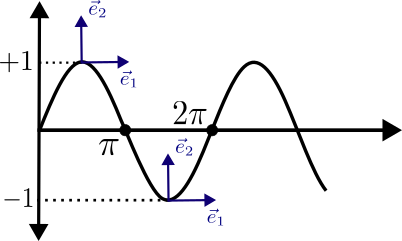
\includegraphics[width=0.35\textwidth]{FOTOS/ejemplo_H_2.png}
    \end{wrapfigure}
$$
\left \{ 
\begin{array}{cc}
     t\in (0,\pi):\ K(t)<0& \text{\parbox{4cm}{La curva gira en el sentido que marca $\mathbf{e_2}$}} \\\\

     
    t\in (\pi,2\pi):\ K(t)>0& \text{\parbox{4cm}{La curva gira en el sentido que marca $-\mathbf{e_2}$}}\\
\end{array}
\right .
$$
\WFclear
\textbf{Observación:} Para ciertos valores de $t$, la curvatura se puede \emph{anular}. Un \emph{punto de inflexión} es aquel en el que ocurre que $K=0$ y $K'=0$.
\end{mybox}

\subsection{Radio de curvatura}
\begin{mybox}
    Diremos que el \textbf{radio de curvatura} en un punto con $K(t)\neq 0$ se define como:
    $$
    \boxed{\rho (t)=\frac{1}{|K(t)|}}
    $$
\end{mybox}
\begin{wrapfigure}{l}{0.25\textwidth}
        \centering
        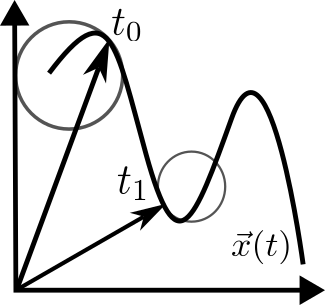
\includegraphics[scale=.4]{FOTOS/radio.png}
\end{wrapfigure}

Para el caso anterior de $x(t)=r\cos{t}, \  y(t)=r\sin{t}$; $\rho(t)=r\equiv$ constante. Geométricamente, $\rho(t)$ representa el \emph{radio instantáneo de una circunferencia} que aproxima \emph{cuadráticamente} la curva en un punto $t$.\\
\WFclear
\subsection{Sistema de Frenet en parametrización natural}

Dada nuestra curva $\mathbf{x}(S)=(x(S),y(S))$ en $\mathbb{R}^2$ en términos del parámetro privilegiado $S$, nuestro sistema de Frenet se construye de la siguiente forma:
\begin{equation*}
\begin{split}
    \left \{ \begin{array}{ccc}
      \mathbf{e_1}   &=&\dot{\mathbf{x}}(S)=(\dot{x}(S),\dot{y}(S))  \\
      \mathbf{e_2}   &=&(-\dot{y}(S),\dot{x}(S)) 
    \end{array} \right . \implies K(S)=\dot{\mathbf{e_1}}(S)\cdot \mathbf{e_2}(S)&=-\ddot{x}(S)\dot{y}(S)+\ddot{y}(S)\dot{x}(S)\\
                                                                     K(t)&=\dot{x}(S)\ddot{y}(S)-\ddot{x}(S)\dot{y}(S)
\end{split}
\end{equation*}
(Resulta más sencillo calcular la curvatura en parametrización natural).
\subsection{Interpretación geométrica de la curvatura en $\mathbb{R}^2$}
Sea $\mathbf{x}:I\subseteq\mathbb{R}\longrightarrow \mathbb{R}^2$ de clase $C^r\ , \ r\ge 2$, escrita en términos del parámetro natural.\\

\begin{wrapfigure}{l}{0.4\textwidth}  
    \centering
    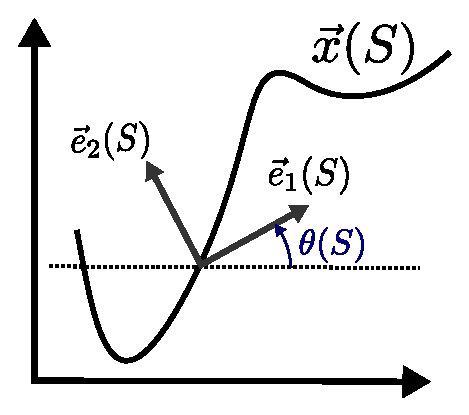
\includegraphics[scale=.8]{FOTOS/interpretacion.eps}
\end{wrapfigure}

$\theta (S)$ es el ángulo que forma el primer vector del sistema de Frenet, que coincide con $\dot{\mathbf{x}}(S)$, con el eje horizontal. Recordamos que estas derivadas en términos de $S$ cumplen que $||\dot{\mathbf{x}}(S)||=1$, por lo que 
$$
\dot{x}(S)^2+\dot{y}(S)^2=1
$$

Además, si descomponemos este vector velocidad en términos de sus proyecciones horizontales y verticales, obtenemos que
$$
\left \{ 
\begin{array}{ccc}
     \dot{x}(S)&=&\cos{\theta(S)}  \\
     \dot{y}(S)&=&\sin{\theta(S)} 
\end{array}
\right .
$$

Por lo que la curvatura $K(S)$ queda escrita como:
\begin{flalign*}
    K(S)&=\dot{x}\ddot{y}-\ddot{x}\dot{y}&&\\
        &=\cos{\theta(S)}\cdot \cos{\theta(S)}\cdot \dot{\theta}(S)+\sin{\theta(S)}\cdot \dot{\theta}(S)\cdot \sin{\theta(S)}=\dot{\theta}(\cos^2\theta + \sin^2\theta)&&\\
        &\implies \boxed{K(S)=\dot{\theta}(S)}
\end{flalign*}

La curvatura representa la variación del ángulo $\theta$ en términos de la longitud de arco.
\subsection{Reconstrucción de una curva a partir de su curvatura}
Supongamos que conocemos la curvatura $K(S)$ de una curva, donde $S$ es el parámetro natural. Recordemos que $K(S)=\dot{\theta}(S)$, con $\dot{x}=\cos{\theta}$, $\dot{y}=\sin{\theta}$. Entonces,
$$
\theta(S)=\int K(S) \odif{S} + \theta_0 \qquad \text{\parbox{10.5cm}{con una constante de integración asociada a la libertad de rotación.}}
$$
y
$$
\begin{array}{ccc}
     x(S)&=&\int \cos{\theta(S)} \odif{S} + x_0 \\
     y(S)&=&\int \sin{\theta(S)} \odif{S} + y_0
\end{array} \qquad \text{\parbox{9cm}{con $x_0,y_0$ constantes de integración asociadas a la libertad de traslación.}}
$$
\begin{mybox}
    \underline{Ejemplo I:} $K(S)=1/(1+S^2)$. Hallar la curva paramétrica.
    $$
    \theta(S)=\int K(S)\odif{S} = \int \frac{\odif{S}}{1+S^2}=\arctan{S}+\cancelto{0}{\theta_0}
    $$

    \begin{enumerate}
        \item[$\rightarrow$] $x(S)$:
        $$
        x(S)=\int \cos{\theta(S)}\odif{S}=\int \cos[\arctan S]\odif{S}
        $$ 

        Por trigonometría: $\tan{\alpha}=\sin{\alpha}/\cos{\alpha}=\sqrt{1-\cos^2\alpha}/\cos\alpha$, por lo que $\cos \alpha=\sqrt{1/(1+\tan^2 \alpha)}$
        $$
        x(S)=\int \cos[\arctan S]\odif{S}=\int \sqrt{\frac{1}{1+s^2}}\odif{S}=\sinh^{-1}(S)+\cancelto{0}{x_0}
        $$

        \item[$\rightarrow$] $y(S)$:
        \begin{flalign*}  
            y(S)&=\int \sin{\theta(S)}\odif{S}&&\\
                &=\int \sin{\arctan \theta}\odif{S}=\int \frac{S\odif{S}}{\sqrt{1+S^2}}=\sqrt{1+S^2}+\cancelto{0}{y_0}
        \end{flalign*}
    \end{enumerate}
    
    Finalmente:
    $$
    \left \{ 
    \begin{array}{ccc}
         x(S)&=&\sinh^{-1}(S)  \\
         y(S)&=&\sqrt{1+S^2} 
    \end{array}
    \right . 
    $$
     \begin{wrapfigure}{r}{0.25\textwidth} 
        \centering
        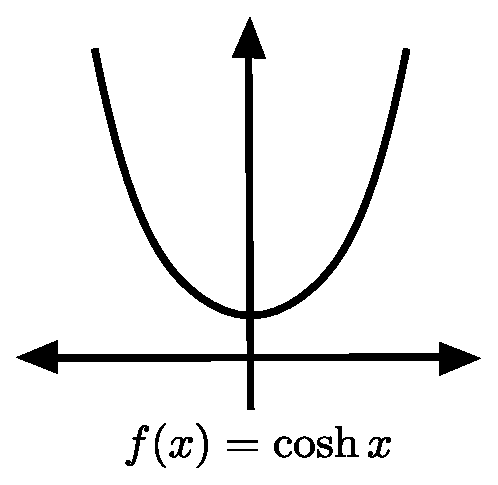
\includegraphics[scale=.45]{FOTOS/catenaria.eps}
    \end{wrapfigure}
    $$
    \mathbf{x}(S)=\left (\sinh^{-1}(S),\sqrt{1+S^2} \right )
    $$
   
    Representar esta curva mediante este parámetro es complicado, por lo que en este caso es útil utilizar una reparametrización.
    $$
    t=\sinh^{-1}(S)\implies \sinh{t}=S \ , \ \sqrt{1+S^2}=\cosh{t}
    $$
    
\end{mybox}

\section{Fórmulas de Frenet}
 Ya hemos tratado el problema del sistema de Frenet en dos dimensiones e introducido el concepto de curvatura a través de la parametrización natural. En el caso de $\mathbb{R}^3$, nuestro parámetro $S\in I$ define la curva como 
 $$
 S\longmapsto \mathbf{x}(S)=(x(S),y(S),x(S))
 $$
 y nuestro sistema de Frenet toma una forma sencilla, porque $||\dot{\mathbf{x}}(S)||=1$.
 $$
 \left \{
 \begin{array}{ccc}
      \mathbf{e_1}(S)&=&\dot{\mathbf{x}}(S)  \\
      \mathbf{e_2}(S)&=&\ddot{\mathbf{x}}(S)/||\ddot{\mathbf{x}}(S)||\\
      \mathbf{e_3}(S)&=&\mathbf{e_1}(S)\wedge \mathbf{e_2}(S)=\frac{\dot{\mathbf{x}}(S)\wedge \ddot{\mathbf{x}}(S)}{||\ddot{\mathbf{x}}(S)||}
 \end{array}
 \right .
 $$

 La notación clásica para el \emph{triedro de Frenet} es:
 \begin{center}
\begin{tabular}{cccc}
     $\mathbf{t}(S)=\mathbf{e_1}$ &:& Vector& \emph{tangente unitario}.\\
     $\mathbf{p}(S)=\mathbf{e_2}$ &:& Vector& \emph{normal principal}.\\
     $\mathbf{b}(S)=\mathbf{e_3}$ &:& Vector& \emph{binormal}.\\
\end{tabular}
\end{center}


\begin{wrapfigure}{l}{0.35\textwidth}
    \centering
    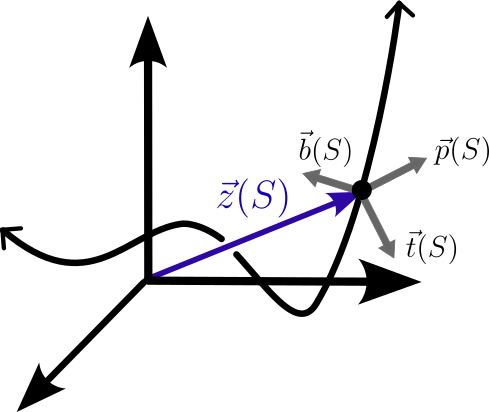
\includegraphics[scale=.4]{FOTOS/frenet_3d.png}
\end{wrapfigure}

Se puede ver de forma muy sencilla que, para $\mathbf{x}\in \mathbb{R}^3$ y un cierto $S$ fijo, $\mathbf{x}(S),\mathbf{t}(S),\mathbf{p}(S),\mathbf{b}(S)$ quedan totalmente fijados. Entonces, para ese punto de coordenadas $\mathbf{z}(S)=(x(S),y(S),z(S))$, los vectores del triedro de Frenet forman tres planos, llamados \emph{normal, rectificante }y \emph{osculador}, que quedan determinados respectivamente por:
$$
\begin{array}{c}
     (\mathbf{z}-\mathbf{x}(S))\cdot \mathbf{t}=0  \\
     (\mathbf{z}-\mathbf{x}(S))\cdot \mathbf{p}=0  \\
     (\mathbf{z}-\mathbf{x}(S))\cdot \mathbf{b}=0
\end{array}
$$
\begin{wrapfigure}{r}{0.3\textwidth}
    \centering
    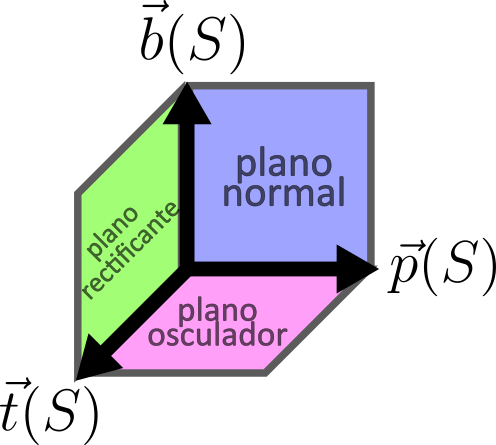
\includegraphics[scale=.4]{FOTOS/planos_triedro.png}
\end{wrapfigure}
En el caso de una curva en $\mathbb{R}^3$, recordamos que tenemos dos curvaturas:
$$
\begin{array}{ccccc}
    K_1(S)&\equiv& \underbrace{K(S)}_{(>0)}  & :&\text{\underline{curvatura}}\\\\
    K_2(S)&\equiv &\tau(S)   &:& \text{\underline{torsión}}
\end{array}
$$

$$
\left ( \begin{array}{c}
     \dot{\mathbf{t}}(S)  \\
     \dot{\mathbf{p}}(S)  \\
     \dot{\mathbf{b}}(S)
\end{array} \right )=\left ( \begin{array}{ccc}
     0&K(S) &0 \\
     -K(S)&0 &\tau (S) \\
     0&-\tau (S) &0
\end{array} \right ) \left ( \begin{array}{c}
     \mathbf{t}(S)  \\
     \mathbf{p}(S)  \\
     \mathbf{b}(S)
\end{array} \right )
$$

La forma explícita de la curvatura y la torsión es:
\begin{enumerate}
    \item[(i)] $K(S)=K_1(S)=$
    $\dot{\mathbf{e}}_1(S)\cdot \mathbf{e}_2(S)=(\ddot{\mathbf{x}}(S)\cdot \ddot{\mathbf{x}}(S))/||\ddot{\mathbf{x}}(S)||=||\ddot{\mathbf{x}}(S)||>0$.
    $$
    \boxed{K(S)=||\ddot{\mathbf{x}}(S)||}
    $$ 

    \item[(ii)] $\tau(S)=K(S)=\dot{\mathbf{e}}_2(S)\cdot \mathbf{e}_3(S)$

    \begin{gather*}
        \mathbf{e_2}=\frac{\ddot{\mathbf{x}}}{||\ddot{\mathbf{x}}||}\implies \dot{\mathbf{e}}_2=\dddot{\mathbf{x}}(S)\cdot \frac{1}{||\ddot{\mathbf{x}}(S)||}+\ddot{\mathbf{x}}(S)\cdot \dv{}{S}\left ( \frac{1}{||\ddot{\mathbf{x}}||} \right ) \\
        \text{pero } \ddot{\mathbf{x}}(S)=\mathbf{e}_2\cdot ||\ddot{\mathbf{x}}(S)||
    \end{gather*}
    es decir, el término de la derivada del módulo no contribuye, quedando únicamente la tercera derivada.
    $$
    \tau(S)=\dot{\mathbf{e}}_2\cdot \mathbf{e}_3=\dot{\mathbf{e}}_2\cdot (\mathbf{e}_1 \wedge \mathbf{e}_2)=\frac{\dddot{\mathbf{x}}(S)}{||\ddot{\mathbf{x}}(S)||}\cdot (\mathbf{e}_1 \wedge \mathbf{e}_2)
    $$
    $$
    \boxed{\tau(S)=\frac{\det{\dot{\mathbf{x}},\ddot{\mathbf{x}},\dddot{\mathbf{x}}}}{||\ddot{\mathbf{x}}||^2}}
    $$
    luego tenemos que $||\ddot{\mathbf{x}}||\neq 0$
\end{enumerate}

Se define el \emph{vector de curvatura} como:
$$
\boxed{\mathbf{K}(S)=K(S)\cdot \mathbf{p}(S)} \ ,
$$
el \emph{centro de curvatura} (para cada punto de la curva) como:
$$
\boxed{\mathbf{x}_{cc}(S)=\mathbf{x}(S)+\frac{1}{K(S)}\mathbf{p}(S)}
$$
y el \emph{radio de curvatura} como:
$$
\boxed{\rho(S)=\frac{1}{K(S)}}
$$

Hasta este punto, todo este desarrollo se aplica para la parametrización natural, especialmente simple por la condición de $||\dot{\mathbf{x}}(S)||=1$. En casos de la parametrización \emph{arbitraria}, se arrastran términos de $||\dot{\mathbf{x}}(S)||=1$ debido a su no unitariedad.\\

En este caso, el triedro de Frenet es:
\begin{gather*}
    \mathbf{e}_1(t)=\frac{\mathbf{x'}(t)}{||\mathbf{x'}(t)||}\equiv \mathbf{t}(t)\\
    \mathbf{e}_3(t)=\frac{\mathbf{x'}(t)\wedge \mathbf{x''}(t)}{||\mathbf{x'}(t)\wedge \mathbf{x''}(t)||}\equiv \mathbf{b}(t)\\
    \mathbf{e}_2(t)=\mathbf{e}_3\wedge \mathbf{e}_1=\mathbf{b}(t)\wedge \mathbf{t}(t)\equiv \mathbf{p}(t)
\end{gather*}

Para calcular la curvatura y la torsión, recordamos que:
\begin{align*}
    K(S)=||\ddot{\mathbf{x}}(S)||&:&\text{\parbox{7cm}{Como se trata de un cambio de variable: $\dv*{}{S}=1/||\mathbf{x'}||\dv*{}{t}$}}
\end{align*}
\begin{enumerate}
    \item[$\xlongrightarrow{1}$]$\dot{\mathbf{x}}(S)=\dv{\mathbf{x}}{S}=\frac{1}{||\mathbf{x'}||}\dv{\mathbf{x}}{t}=\frac{\mathbf{x'}}{||\mathbf{x'}||}$ 

    \item[$\xlongrightarrow{2}$]$\ddot{\mathbf{x}}(S)=\dv{\dot{\mathbf{x}}}{S}=\frac{1}{||\mathbf{x'}||} \left ( \dv{}{t}\left ( \frac{\mathbf{x'}}{||\mathbf{x'}||} \right ) \right )=\frac{\mathbf{x''}}{||\mathbf{x'}||^2}+\mathbf{x'}\cdot \frac{1}{||\mathbf{x'}||} \dv{}{t}\left ( \frac{1}{||\mathbf{x'}||} \right )$
\end{enumerate}

Utilizando los cálculos anteriores,
$$
K(t)=\frac{||\mathbf{x'}(t)\wedge \mathbf{x''}(t)||}{||\mathbf{x'}(t)||^3} \qquad , \qquad \tau(t)=\frac{\det{\dot{\mathbf{x}},\ddot{\mathbf{x}},\dddot{\mathbf{x}}}}{||\mathbf{x'}(t)\wedge \mathbf{x''}(t)||^2}
$$

\subsection{Curvas planas en $\mathbb{R}^3$}
Una curva plana es aquella que está \emph{contenida en un plano} de $\mathbb{R}^3$. Eso significa que uno de los vectores del triedro de Frenet no se está moviendo, en este caso $\mathbf{b}(S)$; es decir, es \emph{constante}.

El trabajar con una curva plana hace que se cumpla que $(\mathbf{x}(S)-\mathbf{x}(0))\cdot \mathbf{n}=0$, donde $\mathbf{n}$ es un vector normal al plano que contiene la curva. Si derivamos esta expresión, obtenemos $\dot{\mathbf{x}}\cdot \mathbf{n}=0$, y $\ddot{\mathbf{x}}\cdot \mathbf{n}=0$, de donde podemos deducir que $\ddot{\mathbf{x}}\sim \mathbf{b} \implies \mathbf{m} \parallel \mathbf{b}(S)$. En consecuencia, $\mathbf{b}\equiv $ const., con $||\mathbf{b}(S)||=1$. \\

Por lo tanto, una curva (en $\mathbb{R}^3$) con curvatura distinta de 0 es plana si y solo si $\tau(S)$ es nula ($\dot{\mathbf{b}}(S)=-\tau(S)\mathbf{p}(S)\equiv 0 \iff \tau(S)=0$).
\begin{mybox}
    \begin{center}
    \fbox{\textbf{Condiciones equivalentes}} \\
    \vspace{0.3cm}
    Una curva es \textbf{plana} si y solo si:
    \begin{gather*}
        \mathbf{b}(S)\equiv \text{constante}
        \iff 
        (\mathbf{x}(S)-\mathbf{x}(0))\cdot \mathbf{n}=0
       \iff 
        \tau(S)=0
    \end{gather*}
    \end{center}
\end{mybox}

\begin{center}
    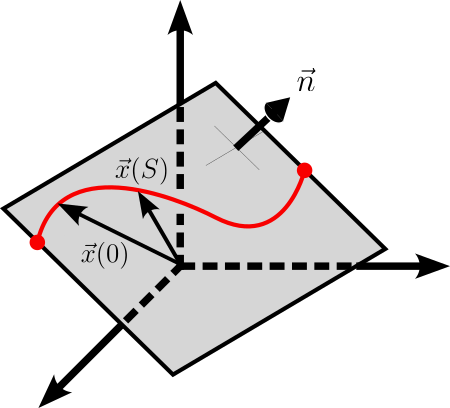
\includegraphics[scale=.65]{FOTOS/curva_plana.png}
\end{center}

